\chapter{PID Controller Design}
\label{chap:PIDControllerDesign}
\abstract{\gls{pid} controller tuning is central in the process control field, but selecting the correct parameters is far from trivial since it needs to take into account multiple considerations such as performance, robustness, topology, etc. This chapter gives an overview of \gls{pid} controller tuning. Analytical tuning methods are presented in order to have the most fundamental mathematical description of a tuning rule. Then, the chapter explores the tuning based on the minimization of a performance criteria which is then applied to integral cost functions. The particular solution to this problem is explored in detail in the next chapter.} 

\section{PID Controller Tuning}
Selecting the appropriate tuning parameters is one of the most important steps in a \gls{pid} based control loop. The selection of the \gls{pid} controller parameters should be made according to the available knowledge of the process dynamics and stated performance specifications in terms of tracking and disturbance attenuation as well as desired robustness. One of the aspects that makes \gls{pid} control especially appealing is the clear physical meaning associated to each one of its parameters.

Numerous studies have been made to develop assignment rules to specify \gls{pid} parameters on the basis of characteristics of the process being controlled. The collected information about the process to be controlled can, in one form or another be assimilated to a model of the process. This can be referred to either as a parametric process model (or, in other words, a form suitable for analyzing and simulating the closed-loop system), or concrete process data and/or measurements that in a suitable way can be directly employed to determine the \gls{pid} controller parameters. There are many representative sources that can be consulted for details on a wide variety of alternative tuning rules  \citep{odwyer2006}.

In what follows, we focus of the most usual existing methods for \gls{pid} tuning. For more in detail explanation on the subject, the reader is encouraged to access other sources such as \citet{VilanovaBook2012}. The material presented in this chapter will serve as the basis to better understand the formulation of the \gls{pid} tuning as a multiobjective optimization problem as proposed in the rest of the book.

\subsection{Analytical Tuning Methods}

Analytical tuning methods are intended to obtain a specified closed-loop time response. This desired closed-loop behavior is defined by a given set of poles or more generally, by defining a reference model. The controller accomplishes its function if the closed-loop mimics this reference model. These approaches were originated by the early works on algebraic controller design in a more generic setting by \citet{ragazzini1958}.

There are a variety of different approaches for the design of the controller, the overall goal is to place the closed-loop poles according to the expected response, in other cases the zeros can also be shaped. However, when dealing with \gls{pid} controllers, the quantity of the poles and zeros is fixed, and therefore there is a limitation in what the controller can achieve.

Given this constraint in the complexity of \gls{pid}, only the dominant poles are considered, and thus only first or second order plant models are taken into account. Then the controller is tuned by re-assigning the system's poles with faster modes. The drawback, however, is that some modes may become uncontrollable due to pole/zero cancellation resulting in performance degradation if they become excited.

The introduction of ideas on algebraic design gave rise to the so called \emph{$\lambda$-tuning} \citep{dahlin68}. It is straightforward to see that for \gls{foptd} and  \gls{soptd} models, \gls{pi} and \gls{pid}
controllers can help achieve the desired performance. The number of poles that can be placed is equal to the number of controller parameters. Therefore, these techniques can be used for process models with the maximum order of 2 if a \gls{pid} controller is selected.

This method, in turn, is closely related to the Smith predictor and the design method based on Internal Model Control (IMC) \citep{riveraetall86}.  In the particular case of a \gls{foptd} process, the IMC controller takes the form of a PI or a \gls{pid} controller depending on the rational approximation used for the time delay.

Nevertheless, there is a limitation on these approaches which is that the poles of the process are canceled possibly leading to undesirable responses in the case of load disturbances, especially for processes with very large time constants. In \citet{chien90}, a modification is presented  that does not cancel the poles of the process, while \citet{Skogestad2003} presents a variation of the IMC controller denominated Simple IMC (SIMC), in which the cancellation is avoided by means of a redefinition of the integral mode for the cases of systems dominated by large time constants.

\citet{chenseborg2002} proposed a modification of the direct synthesis method adapted to disturbance rejection instead of set-point change. Similarly, \citet{shamsu2008} reported that IMC demonstrates sluggish disturbance rejection, especially when the deadtime to time constant ratio is small. To alleviate this problem they proposed an IMC-PID tuning method for improved disturbance rejection. A robust version of this approach is presented by \citet{Vilanova2018}.

One of the advantages of IMC is the introduction of the desired closed-loop time constant, which can be used by operators to manipulate the degree of robustness. \citet{vilanovaJPC2008} proposed a robust IMC based tuning rule for set-point tracking. The tuning introduces two user defined parameters and also provides an automatic tuning rule. 
%
\subsection{Tuning based on Minimization of Performance Criteria}
%
The methods based on the application of optimization techniques are an alternative to the analytical methods. The basic idea is to try to capture different aspects of the desired operation specifying a cost function that is intended to be minimized.

For example, \citet{corripio2001} and \citet{shinskey.1994} present a controller tuning that is found as the solution of an optimization of integral error criteria such as the \gls{ise}, \gls{iae} and \gls{itae}.

Optimization of integral criteria for deriving tuning rules were started by \citet{lopez1967} and \citet{Rovira1969a}, where tunings are provided for load disturbance rejection and set-point tracking separately. When is not clear which mode of operation is more predominant or only \gls{1dof} controllers are available, some tuning methods can be applied where a balanced operation is considered but at the same time, is the solution of an optimization problem \citep{Arrieta2010}. Simple tuning rules for different variants of the integral criteria are provided by \citet{zhuang1993}. Rules for unstable and integrating systems can be found in \citet{visioli2001}.

Over the years, greater accessibility to optimization routines and increasing computing power, have given rise to new multiobjective optimization approaches as is presented by \citet{herreros2002}  and \citet{toivonen2006}, where a general tuning approach is tackled but \gls{pid} controllers are used as particular cases.

In spite of the effectiveness of these multiobjective optimization strategies, they rely on the use of fairly complex numerical routines which hinders recognizing appropriate tuning rules based on the solutions. This is explored in more detail in Chapter~\ref{chap:PIDMOOP}
%
\subsection{Tuning Rules for Robustness}
%
Whereas there are some tuning approaches that provide tuning parameters that  affect the system robustness (this is the case, for example of IMC control), their main aim is not to ensure a robust closed-loop system, but to optimize its performance.

Even if their application may result in a control system with some robustness properties, its achievement will always be indirect. On the other hand, in recent years, there has been an increasing interest in including robustness explicitly into the tuning of the controller as one of the main objectives.

The work of \citet{astromhagglun84} which used the gain and phase margin of the closed-loop system was seminal in giving rise to numerous variants and extensions. In this case, the design parameter or specification is directly measuring the desired robustness for the closed-loop system. Later on, \citet{hoetal95} proposed tuning rules for \gls{pid} controllers for gain and phase specifications.

As previously mentioned, it was within the IMC approach that the work of \citet{vilanovaJPC2008} introduced robustness considerations into the autotuning  formulas. Later,  these ideas brought forth a series of works where the robustness was explicitly considered as part of the design and by taking into account the robustness/performance trade-off \citep{alfaroajoc12, alcantara2010, alcantara2013}.

This has evolved in such a way that today it is common use to include a robustness constraint or consideration in whatever approach. One of the measures that has gained more popularity today is the maximum of the sensitivity function (commonly called $M_S$) as a reasonable robustness measure. It is also possible to distinguish between approaches that are attempting to achieve a closed-loop with a particular value of $M_S$ and more flexible approaches providing tuning rules directly parameterized by the target $M_S$ value \citep{arrieta2012, VilanovaBook2012}. 

The robustness constraint has also been incorporated into more elaborated  methods such as the Model Reference Robust Tuning (MoReRT) approach \citep{alfarojopc22}. Such method incorporates a model reference based design within an optimization procedure and with the mentioned robustness constraint. Robust tuning rules are provided for all the most common process dynamics as well as different levels of robustness. It also allows \gls{pid} formulations where the reference and output signals are filtered and considered as parts of the design \citep{alfaroiechr2013}.
%
%
\section{Formalization of PID tuning as a multiobjective optimization problem}
\label{sec:FormPIDMOOP}
\subsection{Cost Function and Constraint Selection}
\label{sec:CostFunSelec}
When dealing with \gls{pid} tuning, it is common to define a metric either to optimize the parameters, or as a measure to check how well the tuning behaves with respect to another set of parameters.

In theory, to formulate the \gls{moo} problem, any cost function may be used. However, it is common to select cost functions that are contradictory to each other, which is something that arises naturally when dealing with real designs.

For example, in \citet{SabinaSanchez2017} the \gls{iae} and the \gls{tv} are used as contradictory cost functions. \gls{tv} represents the control effort and is related to the robustness of the closed-system, therefore, using these two cost functions, the compromise is made between performance and robustness. Something similar is done in \citet{Pierezan2014}, where a particle swarm optimization technique is applied to the tuning of \gls{pid} controllers for a robotic manipulator. In \citet{Zhou2018} also a two objectives optimization is done with similar cost functions, the difference consist in that a multivariable control loop is tackled at the same time using a compound weight sum of an \gls{iae} metric for three setpoints and a function related to the energy consumption based on the variation of the input variables.

The cost function does not necessarily have to conform to an integral function. For example, in \citet{Abbas1995} the cost functions are the percent overshoot  and the rise time, but the authors also indicate that the settling time and the maximum controller output can also be considered. A more classical approach takes into account frequency domain measures such as phase and gain margins \citep{astromhagglun84,hoetal95}. In \citet{Huang2008a} the $\cal{ H}_\infty$ norm is used in different frequency bands of different sensitivity functions to define several cost functions which are then used in a multi-objective approach.

Other authors tries to combine integral cost functions with other time domain measures, as in \citet{Chiha2012} where the settling time, overshoot, rise time, \gls{iae}, \gls{ise} and \gls{itae} are taken into account in a weighted sum and optimized using an Ant Colony algorithm approach.

Definitively, the selection of the cost function is a widely open subject and it entirely depends on the necessity of the task at hand. According to \citet{Shinskey2002}, the main objective of a process controller is to mitigate the effects of load disturbances thus confining setpoint changes response to secondary importance. The same author states that: \begin{quote}
	``minimum \gls{iae} is a preferred criterion that includes integral error and penalizes continued cycling. Minimum-\gls{iae} tuning also tends to be consistent with minimum error.''
\end{quote}
%

Following this reasoning, in this book we propose to use integral cost functions to measure control performance with respect to input and output disturbances and setpoint changes in a multi-objective framework, taking the maximum sensitivity as a constraint to find the optimal controller tuning.

The controller is considered to be a \gls{2dof} \gls{pid} controller. Even with this topology, the cost functions that are a result of considering all three sources of disturbances are contradictory because minimizing one of them does not minimize the other functions. In fact, you may find that the optimal controller for one cost function yields to the maximum value of other function. These details are covered in Section~\ref{sec:MOOPForm} where the multi-objective framework is stated.

\subsection{PID tuning problem formulation for integral cost functions}
\label{sec:CostProbPID}
A feedback control system like the one shown in %
\begin{figure}[b]
	\centering
	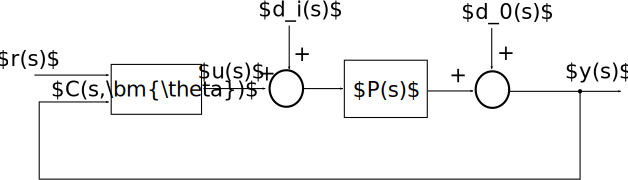
\includegraphics[width=0.85\columnwidth]{Ch4bloques}%pretex=\scriptsize,
	\caption{Feedback control loop.}% 
	\label{fig:bloques}%
\end{figure}
%
Figure~\ref{fig:bloques}, is designed to maintain certain relationships between the process output $y(s)$ and the reference input $r(s)$. For such tasks, the difference between those signals is used to compute the control signal $u(s)$ needed in order to achieve $y(s) \approx r(s)$. 

In Figure.~\ref{fig:bloques}, $C(s,\bm{\theta})$ is the \gls{2dof} \gls{pid} controller with parameters:
\begin{equation*}
\bm{\theta}=\left[	\begin{tabular}{cccc} \gls{kp} & \gls{ti} & \gls{td} & \gls{beta}	\end{tabular}\right]^T,
\end{equation*}
%
where \gls{kp} is the proportional gain, \gls{ti} is the integral time constant, \gls{td} is the derivative time constant, \gls{beta} is the weight on the reference signal. \gls{plan} represents the controlled process, modeled as a \gls{soptd} plant, with a transfer function of the form:
\begin{equation}  %inclusión de ecuaciones
P(s) =  \frac{K e^{-Ls}}{(T s+1)(a T s+1)},
\label{eq:plantaX}
\end{equation}
%
where \gls{k}, \gls{l} and \gls{t} correspond to the static gain, the time delay and main time constant respectively. The other pole of the system is represented with a time constant that is fraction of $T$, therefore $0 \leq a \leq 1$. \gls{di} represent the input disturbance while \gls{do} is the output disturbance.

%El diagrama de bloques de un controlador PI de dos grados de libertad se muestra en la Figura \ref{fig:controlador}. 
%
The relationship between the control signal, the reference and the process output is given by:
%
\begin{equation}  %inclusión de ecuaciones
\gls{u} = \gls{contr} \gls{r} - \gls{conty} \gls{y},
\label{us}
\end{equation}
%
where the part applied to the reference signal is given by:
%
\begin{equation}  %inclusión de ecuaciones
\gls{contr}=  \gls{kp}\left({\gls{beta} + \frac{1}{\gls{ti} s}+ \gls{gamma} \frac{\gls{td} s}{\gls{alpha} \gls{td} s +1}}\right),
\label{eq:cr}
\end{equation}
%
and the part applied to the process output is:
%
\begin{equation}  %inclusión de ecuaciones
\gls{conty}=  \gls{kp}\left({1 + \frac{1}{\gls{ti} s}+\frac{\gls{td} s}{\gls{alpha} \gls{td} s +1} }\right).
\label{eq:cy}
\end{equation}

It is common to set $\gls{alpha}=0.1$ and $\gls{gamma}=0$. For this reason, the controller parameter vector is give as $\gls{theta}=[\begin{tabular}{cccc} \gls{kp} & \gls{ti} & \gls{td} &\gls{beta} \end{tabular}]^T$. A detailed description of the controller transfer function is presented in 
\begin{figure}[tb]
	\centering
	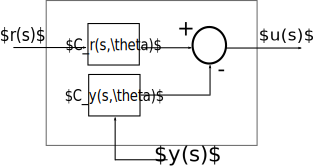
\includegraphics[width=0.7\columnwidth]{Ch4controlador}
	\caption{Representation of the \gls{2dof} controller.}
	\label{fig:Ch4controlador}
\end{figure}
%
Figure~\ref{fig:Ch4controlador}.

To simplify the analysis, the model of the controlled process is normalized:
%
\begin{equation*}
\hat{s}= Ts, \ \tau_0=  \displaystyle\frac{L}{T}, \ \tau_i=  \displaystyle\frac{T_i}{T}, \ \tau_d = \frac{T_d}{T}, \ \kappa_p= K_p K.
\end{equation*}  %inclusión de ecuaciones

Then the normalized parameters of the controller become $\bm{\theta}=\left[\kappa, \tau_i, \tau_d, \beta\right]^T$.
%
and the response of the controlled system is computed as: 
%%
\begin{equation} 
 y(\hat{s})= y_r(\hat{s}) + y_{di}(\hat{s}) + y_{do}(\hat{s}),
\label{ys}
\end{equation}
%
where $y_r(\hat{s})$, is the output response to a change in the setpoint $r(\hat{s})$, $y_{di}(\hat{s})$ is the response to a change in the input disturbance signal $d_i(\hat{s})$ and $y_{do}(\hat{s})$ is the response to a change in the output disturbance signal $d_o(\hat{s})$. From Figure~\ref{fig:bloques} and Figure~\ref{fig:Ch4controlador}, these signals can be computed as:
%
\begin{align*}
 y_r(\hat{s}) &= \frac{P(\hat{s}) C_r(\hat{s},\bm{\theta}) }{1 + P(\hat{s}) C_y(\hat{s},\bm{\theta})} r(\hat{s})\\
y_{di}(\hat{s}) &=  \frac{C_r(\hat{s},\bm{\theta})}{1 + P(\hat{s}) C_y(\hat{s},\bm{\theta})} d_i(\hat{s}) \\%
y_{do}(\hat{s}) &= \frac{1}{1 + P(\hat{s}) C_y(\hat{s},\bm{\theta})} {d_o(\hat{s})}
\label{ytot}
\end{align*}

%Dada \eqref{ys}, la respuesta de salida del lazo cerrado ante un cambio en el valor deseado puede ser ajustada a través del controlador de valor deseado $C_r(\hat{s},\theta)$, independientemente de cambios en la perturbación de entrada o en la de salida. Los parámetros de $C_r(\hat{s},\theta)$ y $C_y(\hat{s},\theta)$ son los mismos con un grado de libertad \cite{apuntescontrol}.

Robustness is an indication of the relative stability of the controlled system and it measures the ability of the controller to keep the closed-loop stable despite the variation in the process dynamics. A metric of the degree of relative stability is the maximum sensitivity \gls{ms} given by:
%
\begin{equation}  %inclusión de ecuaciones
\gls{ms}=  \max_\omega \left\{ \frac{1}{\left |{1 + C_y(j\omega ) P(j\omega )}\right |}\right\} 
\label{Ms}
\end{equation}

As it is widely established, the controller tuning can be solved as a multi-objective optimization problem~\citep{Gambier2007}. One common indicator of performance, is the \gls{iae} given by:
%
\begin{equation}  %inclusión de ecuaciones
J(\bm{\theta})=\int_0^\infty \left |{e(t,\bm{\theta})}\right | dt.
\label{IAE}
\end{equation}

The error signal $e(t, \bm{\theta})$ is calculated using:
%
\begin{equation}  %inclusión de ecuaciones
e(t,\bm{\theta})=r(t)-y(t,\bm{\theta}).
\label{error}
\end{equation}

When \eqref{IAE} is computed for a step change in the reference signal, the cost function becomes $J_r(\bm{\theta})$; for an input disturbance response, the function is defined as $J_{di}(\bm{\theta})$ and finally, for an output disturbance response, the cost function is named as $J_{do}(\bm{\theta})$.

When the output of the plant is disturbed only by the step change in $d_i(\hat{s})$, the error signal then becomes:
\begin{equation}  %inclusión de ecuaciones
e_d(t)=-y_{di}(t)
\label{per}.
\end{equation}

And then, the cost function $J_{di}(\bm{\theta})$ is computed as:
\begin{equation}  %inclusión de ecuaciones
J_{di}(\bm{\theta})= \int_0^\infty  \left |-{y_{di}(t,\bm{\theta})}\right | dt,
\label{perin}
\end{equation}

On the other hand, if the disturbance comes only from a step signal in $d_o(\hat{s})$, the cost function that has to be computed is $J_{do}(\bm{\theta})$ as:
%
\begin{equation}  %inclusión de ecuaciones
J_{do}(\bm{\theta})= \int_0^\infty  \left |-{y_{do}(t,\bm{\theta})}\right | dt.
\label{perout}
\end{equation}	
%

Finally, if the setpoint is the only source of disturbance for the plant, the corresponding cost function $J_r(\bm{\theta})$ is computed as:
\begin{equation}  %inclusión de ecuaciones
J_r(\bm{\theta})=\int_0^\infty \left |r(t)-y_r(t,\bm{\theta})\right | dt.
\label{eq:Jr}
\end{equation}
%

The problem of minimizing $J_r(\bm{\theta})$, $J_{di}(\bm{\theta})$ and $J_{do}(\bm{\theta})$ at the same time can be posed as a \gls{moo} problem. In addition, since in an industrial environment the robustness is very important, the obtained parameters are constrained to always satisfy  $\gls{ms} \leq M_{s,max}$, where $M_{s,max}$ is the allowed limit of the maximum sensitivity. The combined cost function (vector of cost functions) then becomes:
%
\begin{equation}  %inclusión de ecuaciones
\textbf{J}(\bm{\theta})=\left[J_{di}(\bm{\theta}), J_{do}(\bm{\theta}), J_{r}(\bm{\theta})\right]^T,
\label{eq:Jtotal}
\end{equation}
%
and solved by finding all possible optimal solutions of:
%
\begin{equation}  %inclusión de ecuaciones
\begin{gathered}
\textbf{J}(\bm{\theta}^*) = \min_{\bm{\theta}} \textbf{J}(\bm{\theta}),\\
\text{s.t.} \quad  M_s \leq M_{s,max}
\end{gathered}
\label{eq:probmoo}
\end{equation}

In general, it is not possible to find a set of parameters $\bm{\theta}$ that minimizes all those three functions at the same time. This impossible point where all the cost functions are optimal is called the utopia point. As it names states, the utopia point is impossible to reach because optimizing one of the cost function always produces a degradation in the other remaining functions.

The particular cases that are  the closest to the utopia point, are part of what is called the Pareto frontier. This set of possible solutions are considered to be equally optimal because there is no possibility to improve one of the functions without degrading the others.

This means that finding the solution of the control problem does not give a single answer, instead provides a family of optimal controller tunings as will be explored further in the rest of the book.
\bibliographystyle{spbasic}
\bibliography{ReferenciasMulti}